\item What is the equation of the function shown in the graph?

% \resizebox{3in}{!}{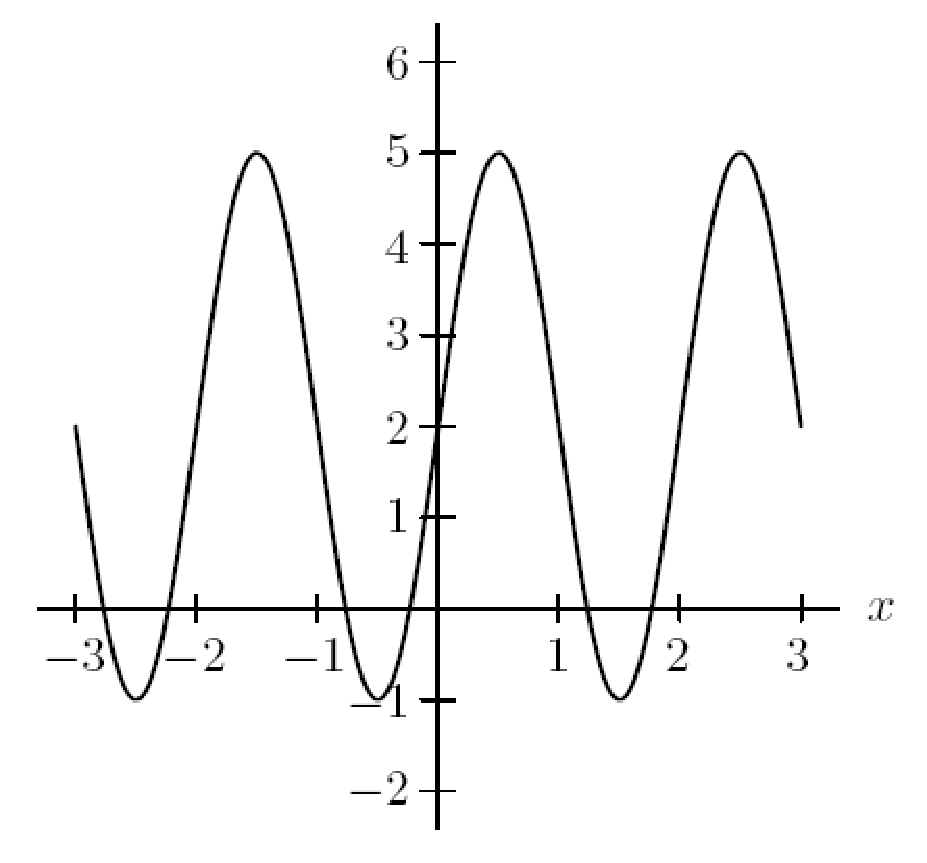
\includegraphics{SVC.01.05.010.ps}}

\begin{minipage}{0.4\columnwidth}
    \begin{enumerate}
        \item $y = 3 \sin (2x)+2$
        \item $y = 3\cos(2x)+2$
        \item $y=3\sin(\pi x)+2$
        \item $y = 3 \cos (\pi x) +2$
        \item $y=3 \sin (\frac{1}{\pi} x) +2$
        \item $y = 3 \cos((\frac{1}{\pi} x)+2)$
    \end{enumerate}
\end{minipage}
\begin{minipage}{0.6\columnwidth}
    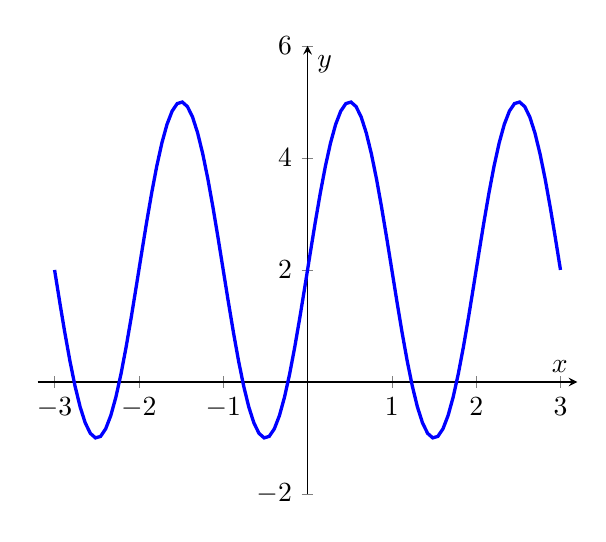
\begin{tikzpicture}
        \begin{axis}[axis lines=center, xlabel={$x$}, ylabel={$y$}, xmin=-3.2, xmax=3.2,
                ymin=-2, ymax=6]
                \addplot[color=blue, very thick,domain=-3:3, samples=100]
                {3*sin(pi*deg(x))+2};
            \end{axis}
    \end{tikzpicture}
\end{minipage}

%by Project MathVote; graph from ConceptTests to accompany Calculus 4th Edition, Hughes-Hallet et al., John Wiley & Sons
